\documentclass[]{article}
\usepackage{lmodern}
\usepackage{amssymb,amsmath}
\usepackage{ifxetex,ifluatex}
\usepackage{fixltx2e} % provides \textsubscript
\ifnum 0\ifxetex 1\fi\ifluatex 1\fi=0 % if pdftex
  \usepackage[T1]{fontenc}
  \usepackage[utf8]{inputenc}
\else % if luatex or xelatex
  \ifxetex
    \usepackage{mathspec}
  \else
    \usepackage{fontspec}
  \fi
  \defaultfontfeatures{Ligatures=TeX,Scale=MatchLowercase}
\fi
% use upquote if available, for straight quotes in verbatim environments
\IfFileExists{upquote.sty}{\usepackage{upquote}}{}
% use microtype if available
\IfFileExists{microtype.sty}{%
\usepackage{microtype}
\UseMicrotypeSet[protrusion]{basicmath} % disable protrusion for tt fonts
}{}
\usepackage[margin=1in]{geometry}
\usepackage{hyperref}
\hypersetup{unicode=true,
            pdftitle={Final Project Report - Predicting West Nile},
            pdfauthor={Group 3 - Camron Pearce, Amy Fox, Alyssa Melvin, Kayla Williams},
            pdfborder={0 0 0},
            breaklinks=true}
\urlstyle{same}  % don't use monospace font for urls
\usepackage{longtable,booktabs}
\usepackage{graphicx,grffile}
\makeatletter
\def\maxwidth{\ifdim\Gin@nat@width>\linewidth\linewidth\else\Gin@nat@width\fi}
\def\maxheight{\ifdim\Gin@nat@height>\textheight\textheight\else\Gin@nat@height\fi}
\makeatother
% Scale images if necessary, so that they will not overflow the page
% margins by default, and it is still possible to overwrite the defaults
% using explicit options in \includegraphics[width, height, ...]{}
\setkeys{Gin}{width=\maxwidth,height=\maxheight,keepaspectratio}
\IfFileExists{parskip.sty}{%
\usepackage{parskip}
}{% else
\setlength{\parindent}{0pt}
\setlength{\parskip}{6pt plus 2pt minus 1pt}
}
\setlength{\emergencystretch}{3em}  % prevent overfull lines
\providecommand{\tightlist}{%
  \setlength{\itemsep}{0pt}\setlength{\parskip}{0pt}}
\setcounter{secnumdepth}{0}
% Redefines (sub)paragraphs to behave more like sections
\ifx\paragraph\undefined\else
\let\oldparagraph\paragraph
\renewcommand{\paragraph}[1]{\oldparagraph{#1}\mbox{}}
\fi
\ifx\subparagraph\undefined\else
\let\oldsubparagraph\subparagraph
\renewcommand{\subparagraph}[1]{\oldsubparagraph{#1}\mbox{}}
\fi

%%% Use protect on footnotes to avoid problems with footnotes in titles
\let\rmarkdownfootnote\footnote%
\def\footnote{\protect\rmarkdownfootnote}

%%% Change title format to be more compact
\usepackage{titling}

% Create subtitle command for use in maketitle
\newcommand{\subtitle}[1]{
  \posttitle{
    \begin{center}\large#1\end{center}
    }
}

\setlength{\droptitle}{-2em}

  \title{Final Project Report - Predicting West Nile}
    \pretitle{\vspace{\droptitle}\centering\huge}
  \posttitle{\par}
    \author{Group 3 - Camron Pearce, Amy Fox, Alyssa Melvin, Kayla Williams}
    \preauthor{\centering\large\emph}
  \postauthor{\par}
      \predate{\centering\large\emph}
  \postdate{\par}
    \date{December 7, 2018}


\begin{document}
\maketitle

\emph{Our GitHub is accessible
\href{https://github.com/camronp/predicting_wn}{here}.}

\hypertarget{aim}{%
\section{Aim}\label{aim}}

To build a predictive model that incorporates weather to provide early
indications of the risk of WNV infection in Chicago, Illinois.

\hypertarget{datasets-used}{%
\section{Datasets Used}\label{datasets-used}}

We used mosquito trap data from Chicago, Illinois which we found in a
Kaggle competition website. We had some issues trying to find usable
data for Colorado or other regions in the US, so we settled with this
particular dataset. This particular data set had information on the year
and week the trap was set and collected, the test ID, the trap number,
the block or location where the trap was set, the type of trap, the test
date of the mosquito specimens, the number of mosquitos tested, the
result of the mosquitos that were tested, the species identification of
the mosquitos, and the latitude and longitude of the trap locations. A
majority of the traps set were Gravid traps which are designed to catch
\emph{Culex} species that are capable of transmitting the West Nile
virus. We wanted to calculate the proportion of positive mosquitos
collected each week and a snapshot of the resulting final data set is
below.

\begin{longtable}[]{@{}lllll@{}}
\toprule
week & year & \# of WNV mosquitoes & total \# of mosquitoes & ratio of
WNV mosquitoes\tabularnewline
\midrule
\endhead
23 & 2016 & 0 & 139 & 0.0000000\tabularnewline
23 & 2017 & 0 & 550 & 0.0000000\tabularnewline
23 & 2018 & 50 & 1127 & 0.0443656\tabularnewline
24 & 2016 & 0 & 1138 & 0.0000000\tabularnewline
24 & 2017 & 44 & 533 & 0.0825516\tabularnewline
24 & 2018 & 2 & 1350 & 0.0014815\tabularnewline
\bottomrule
\end{longtable}

When we were researching things that may influence WNV infection of
mosquitos, we found a paper that explained soil temperature,
precipitation, wind speed, and relative humidity have some sort of
association with WNV infected mosquitos in Northern Greece. With that in
mind, we chose NOAA weather data. We had quite a few columns which had
mostly NAs so we wanted to filter it down to just precipitation for this
particular project. We grouped the data by year and week and found the
mean precipitation for that week and year.

\begin{longtable}[]{@{}lll@{}}
\toprule
year & week & avg precipitation\tabularnewline
\midrule
\endhead
2016 & 18 & 0.3146328\tabularnewline
2016 & 19 & 0.2867082\tabularnewline
2016 & 20 & 0.1035765\tabularnewline
2016 & 21 & 0.1628283\tabularnewline
2016 & 22 & 0.2074008\tabularnewline
2016 & 23 & 0.0589617\tabularnewline
\bottomrule
\end{longtable}

We wanted to find soil temperature data as well. We found soil data in
an area that was near Illinois, but about 20 miles away. When we spoke
with professionals in the field, we were told it would be beneficial to
filter our data to average soil temperature in 4 inch sod and average
soil temperature in 2 inch bare soil. We also grouped this data by week
and year and found the average for those weeks.

\begin{longtable}[]{@{}llll@{}}
\toprule
year & week & avg 4 inch soil temp & avg 2 inch soil temp\tabularnewline
\midrule
\endhead
2016 & 18 & 52.52000 & 53.46000\tabularnewline
2016 & 19 & 58.25714 & 61.61429\tabularnewline
2016 & 20 & 57.68571 & 58.50000\tabularnewline
2016 & 21 & 64.48571 & 71.02857\tabularnewline
2016 & 22 & 70.51429 & 73.05714\tabularnewline
2016 & 23 & 68.65714 & 70.47143\tabularnewline
\bottomrule
\end{longtable}

\hypertarget{how-we-tackled-the-problem}{%
\section{How we tackled the problem}\label{how-we-tackled-the-problem}}

First we had to find the data we wanted to use from various sources. We
then had to clean the data and modify it to a point where we could use
it for what we had planned to do. We then wanted to examine the
relationships among the variables. For this, we used a correlation plot.
Our correlation plot indicates that there is a negative association
between the number of positive WNV mosquitos and average soil
temperature in 4 inch sod, average soil temperature in 2 inch bare soil,
average temperature, and mean precipitation.

\includegraphics{final_report_files/figure-latex/preliminary visualization-1.pdf}
\includegraphics{final_report_files/figure-latex/preliminary visualization-2.pdf}
\includegraphics{final_report_files/figure-latex/preliminary visualization-3.pdf}
\includegraphics{final_report_files/figure-latex/preliminary visualization-4.pdf}
\includegraphics{final_report_files/figure-latex/preliminary visualization-5.pdf}
\includegraphics{final_report_files/figure-latex/preliminary visualization-6.pdf}
\includegraphics{final_report_files/figure-latex/preliminary visualization-7.pdf}

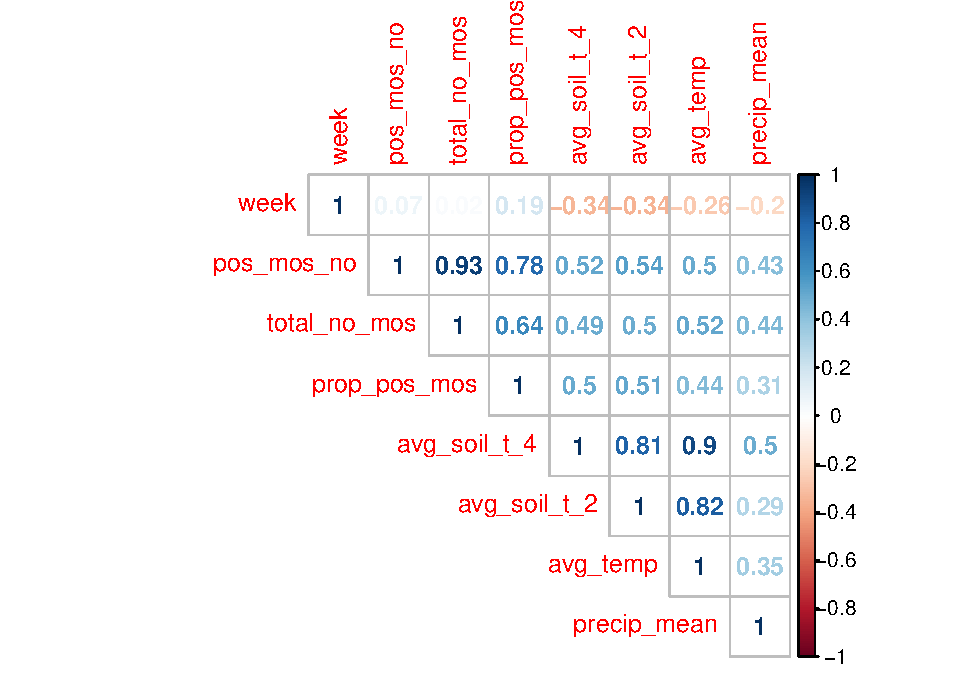
\includegraphics{final_report_files/figure-latex/correlation_plot-1.pdf}

To build a prediction model for proportion of positive mosquitos, we
tested three type of models: a linear prediction model, a regression
tree, and random forest. For the models, we split the data into 2
sections: the first would contains the data collected from 2016 and 2017
to train the datasets, and the second contains the 2018 data to test the
accuracy of the models.

For the linear prediction model we looked at Nick Good's example he used
in class for his running data and attempted something similar. When we
tested the prediction model for week 34 in 2017: 72.1 t4, 74.7 t2, 0.078
precip - the actual proportion should be 0.52. The proportion our model
output is below.

The mean average error for the proportion of positive mosquitoes for the
linear model was also calculated to be 0.1199714.

Decision tree learning looks at multiple observations to predict a
conclusion based off of yes/no decisions about the data.
\includegraphics{final_report_files/figure-latex/regression_tree-1.pdf}
For the regression tree model, the mean average error for the proportion
of positive mosquitoes is be 0.2006875

Random Forest is similar to decision trees, but it is more robust in
that it creates many trees (in the case of our model, 500) and uses the
mean prediction of all of the trees to predict an outcome.

The random forest model, the mean average error for the proportion of
positive mosquitoes is be 0.1227631

\hypertarget{discovery-of-interesting-things}{%
\section{Discovery of Interesting
Things}\label{discovery-of-interesting-things}}

There was a large number of positive WNV tested mosquitos the 30th week
of 2016. The dates for this time were July 25th through July 31st. The
precipitation mean during that time was 0.467 inches. There is a
negative association between the average soil temperatures (in both 2
inch bare soil and in 4 inch sod) and precipitation.

WNV incidence goes up if the daily high temperature in the spring and
early summer is warmer than 81 degrees more often than normal
(ScienceNetLinks, 2018). This is because \textbf{Culex pipiens} will
peak earlier and thus more WNV cases.

For the prediction models it was also interesting that each of the
models chose different variables that they deemed important in
predicting the proportion of positive mosquitoes.

\hypertarget{how-project-fits-into-west-nile-research}{%
\section{How project fits into West Nile
research}\label{how-project-fits-into-west-nile-research}}

West Nile virus is mostly spread to people by mosquito bites. Mosquito
season in North America starts in the summer and continues through fall.
There are no vaccines to prevent or medications to treat West Nile Virus
(WNV) and cases have been reported in all of the US. Most people
infected with WNV do not have symptoms, but about 1 in 5 people who are
infected will develop a fever and other symptoms (CDC, 2018).
Approximately 1 in 150 infected people will develop a serious illness
(CDC, 2018). Since WNV is a virus of public health importance, it's
important to understand its current and future risk factors.
Understanding the risk of WNV infection in the mosquito population will
help us understand the risk of WNV infection in humans and what
prevention methods will need to be communicated during most severe WNV
infection times. Mosquito based surveillance has been a practical and
popular way to estimate the risk of transmission of WNV to people.
Temperature and precipitation play a role in driving mosquito infection
rates and transmission of WNV. Weather conditions and patterns of
meteorological events have important consequences for WNV transmission
as well. High temperatures and low precipitation can often increase WNV
mosquito infection.

\hypertarget{challenges}{%
\section{Challenges}\label{challenges}}

As mentioned earlier, we did have issues finding usable data. We found
quite a bit of information but unfortunately not in files we could use
in R. The Center for Disease Control and Prevention (CDC) has a lot of
information but it is mostly static maps we couldn't find base data for.
Vector Disease Control International also had quite a bit of
information, but again unfortunately no hard data files. For this
reason, and time restraints, is why we settled with Chicago mosquito
trap data we found on the Kaggle competition website. We also had a hard
time conceptualizing exactly what we wanted to predict. We started going
down a hole of collecting a bunch of data and had to quickly realize we
needed to pull back a bit. We had a lot of really great ideas and needed
to decide what would be feasible in the small amount of time we had. We
talked about how this particular project is sometimes an entire thesis
for some students and we only had a few weeks to complete it.

\hypertarget{what-wed-do-differently}{%
\section{What we'd do differently}\label{what-wed-do-differently}}

\begin{itemize}
\tightlist
\item
  Contact Public Health Departments or other entities at the beginning
  for access to data
\item
  Really understand prediction models in R
\item
  Come up with an idea for a prediction model earlier
\item
  Create a ``records'' document to track changes
\item
  Changes and additions to the Shiny app
\item
  Use sepearate ``testing'' notation for markdown chunks
\item
  Annotate code more often
\item
  Overall better communication
\end{itemize}

\hypertarget{references}{%
\subsubsection{References:}\label{references}}

Centers for Disease Control and Prevention (CDC). West Nile virus.
November 28, 2018. Retrieved from:
\url{https://www.cdc.gov/westnile/index.html}

ScienceNetLInks. West Nile Weather. December 10, 2018. Retrieved from:
\url{http://sciencenetlinks.com/science-news/science-updates/west-nile-weather/}


\end{document}
